\documentclass[10pt,mathserif]{beamer}

\usepackage{graphicx,amsmath,amssymb,tikz,psfrag}
\input defs.tex
\setbeamertemplate{blocks}[rounded][shadow]
\usepackage{yfonts}

%% formatting

\mode<presentation>
{
\usetheme{default}
}
\setbeamertemplate{navigation symbols}{}
\usecolortheme[rgb={0.13,0.28,0.59}]{structure}
\setbeamertemplate{itemize subitem}{--}
\setbeamertemplate{frametitle} {
	\begin{center}
	  {\large\bf \insertframetitle}
	\end{center}
}

\newcommand\footlineon{
  \setbeamertemplate{footline} {
    \begin{beamercolorbox}[ht=2.5ex,dp=1.125ex,leftskip=.8cm,rightskip=.6cm]{structure}
      \footnotesize \insertsection
      \hfill
      {\insertframenumber}
    \end{beamercolorbox}
    \vskip 0.45cm
  }
}
\footlineon

\AtBeginSection[] 
{ 
	\begin{frame}<beamer> 
		\frametitle{Outline} 
		\tableofcontents[currentsection,currentsubsection] 
	\end{frame} 
} 

%% begin presentation

\title{\large \bfseries Convex optimization in 20 min, PART I}

\author{Luke\\[3ex]
DHI, CU Boulder}

\date{\today}
 
\begin{document}

\frame{
\thispagestyle{empty}
\titlepage
}

\section{Introduction}
\begin{frame}
\frametitle{One thing that caught my eyes}

Dynamic optimizer — a perceptual video encoding optimization framework (https://netflixtechblog.com/dynamic-optimizer-a-perceptual-video-encoding-optimization-framework-e19f1e3a277f)\\
By Ioannis Katsavounidis\\

\begin{center}
\includegraphics[height=.8\textheight]{figures/dyop.png}
\end{center}
\end{frame}

\begin{frame}
\frametitle{It is becoming popular}
\begin{itemize}\itemsep=12pt
\item Keyword counts in Advances in Neural Information Processing Systems 
\vspace*{0.5em}
\begin{itemize}
\item  (NIPS 2009): 7
\item  (NIPS 2010): 9
\item  (NIPS 2011): 10
\item  (NIPS 2012): 12
\item  (NIPS 2013): 17
\item  (NIPS 2014): 16
\item  (NIPS 2015): 31
\item  (NIPS 2016): 39
\item  (NIPS 2017): 29
\item  (NIPS 2018): 62
\item  (NIPS 2019): 73  $\Leftarrow$
\item  (NIPS 2020): ? 
\end{itemize}
\end{itemize}

\end{frame}

\begin{frame}\frametitle{The one that got away}
\begin{block}{Can you solve this by hand?}
	\[\Huge \int _{0\:}^{\:1}\:e^{\left(sinx\right)}dx\]
\end{block}

	
\end{frame}

\begin{frame}\frametitle{The one that got away}
\begin{block}{Can you solve this by hand?}
\[\Huge \int _{0\:}^{\:1}\:e^{\left(sinx\right)}dx\]
\end{block}
\begin{itemize}
\item Numerical Mathematics 

\end{itemize}

\end{frame}

\begin{frame}\frametitle{The one that got away}
	\begin{block}{Can you solve this by hand?}
		\[\Huge \int _{0\:}^{\:1}\:e^{\left(sinx\right)}dx\]
	\end{block}
	\begin{itemize}
		\item Numerical Mathematics 
		\item Hyperparameter tuning (NP)
	
		
	\end{itemize}
	
\end{frame}

\begin{frame}\frametitle{The one that got away}
	\begin{block}{Can you solve this by hand?}
		\[\Huge \int _{0\:}^{\:1}\:e^{\left(sinx\right)}dx\]
	\end{block}
	\begin{itemize}
		\item Numerical Mathematics 
		\item Hyperparameter tuning (NP)
		\item My understanding of Black box
 
		
	\end{itemize}
	
\end{frame}

\begin{frame}\frametitle{The one that got away}
	\begin{block}{Can you solve this by hand?}
		\[\Huge \int _{0\:}^{\:1}\:e^{\left(sinx\right)}dx\]
	\end{block}
	\begin{itemize}
		\item Numerical Mathematics 
		\item Hypeparameter tuning (NP)
		\item My understanding of Black box
		\item Back-propagation, SGD, work2vec. Seriously? 

	\end{itemize}
	
\end{frame}

\begin{frame}\frametitle{The one that got away}
	\begin{block}{Can you solve this by hand?}
		\[\Huge \int _{0\:}^{\:1}\:e^{\left(sinx\right)}dx\]
	\end{block}
	\begin{itemize}
		\item Numerical Mathematics 
		\item Hyperparameter tuning (NP)
		\item My understanding of Black box
		\item Back-propagation, SGD, work2vec. Seriously? 
		\item "Training ever bigger convnets and LSTMs on ever bigger datasets gets us closer to Strong AI -- in the same sense that building taller towers gets us closer to the moon." -- François Chollet

		
	\end{itemize}
	
\end{frame}

\begin{frame}\frametitle{The one that got away}
	\begin{block}{Can you solve this by hand?}
		\[\Huge \int _{0\:}^{\:1}\:e^{\left(sinx\right)}dx\]
	\end{block}
	\begin{itemize}
		\item Numerical Mathematics 
		\item Hypeparameter tuning (NP)
		\item My understanding of Black box
		\item Back-propagation, SGD, work2vec. Seriously? 
		\item "Training ever bigger convnets and LSTMs on ever bigger datasets gets us closer to Strong AI -- in the same sense that building taller towers gets us closer to the moon." -- François Chollet
		\item There must be a way! Or I could be completely wrong. 
		
	\end{itemize}
	
\end{frame}

\begin{frame}\frametitle{Convex Optimization! The age of reading books is not dead yet. \\
{Theory, Application, Algorithm}}
\begin{center}
\includegraphics[height=.8\textheight]{figures/bv_cvxbook_cover.jpg}
\end{center}
\end{frame}

\begin{frame}\frametitle{I am bored already, and I only care about machine learning}
\begin{block}{Well}
\begin{itemize}
\item Linear regression/ Ridge regression, with Tikhonov regularisation, etc
\item Sparse linear regression with L1 regularisation, such as lasso
\item Support vector machines
\item Parameter estimation in linear-Gaussian time series (Kalman filter and friends)
\item Neural networks
\item Maximum likelihood mixtures of Gaussians
\end{itemize}
\end{block}
\end{frame}



\begin{frame}\frametitle{A little bit of history}
\begin{itemize}
\item Theory (convex analysis): 1900–1970
\item Algorithm: 
\item 1947: simplex algorithm for linear programming (Dantzig)
\item 1960s: early interior-point methods (Fiacco $\&$ McCormick, Dikin)
\item 1970s: ellipsoid method and other sub gradient methods
\item 1980s: polynomial-time interior-point methods for linear programming (Karmarkar 1984)
\item Late 1980s–now: polynomial-time interior-point methods for nonlinear convex optimization (Nesterov $\&$ Nemirovski 1994)
\item Application:
\item Since 1990: many new applications in engineering (control, signal processing, communications, circuit design, machine learning); new problem classes (semidefinite and second-order cone programming, robust optimization)

\end{itemize}

\end{frame}
\begin{frame}\frametitle{Oh, I've seen it before.}
\begin{center}
\includegraphics[height=.6\textheight]{figures/gd.jpeg}
\end{center}

\end{frame}

\begin{frame}\frametitle{OR, this?}
\begin{center}
\includegraphics[height=.6\textheight]{figures/descent_3.png}
\end{center}
\begin{block}{Interested?}

\end{block}
\end{frame}

\begin{frame}\frametitle{OR, this?}
	\begin{center}
		\includegraphics[height=.6\textheight]{figures/descent_3.png}
	\end{center}
	\begin{block}{Are you interested?}
		Fun is over.
	\end{block}
\end{frame}


\begin{frame}\frametitle{Mathematical optimizaiton}
\begin{center}
\includegraphics[height=.8\textheight]{figures/mathopt.png}
\end{center}
\end{frame}

\begin{frame}\frametitle{Least-squares}
\begin{center}
\includegraphics[height=.8\textheight]{figures/leastsqrt.png}
\end{center}
\end{frame}

\begin{frame}\frametitle{Convex optimization problem}
\begin{center}
\includegraphics[height=.8\textheight]{figures/cvopt.png}
\end{center}
\end{frame}

\begin{frame}\frametitle{Can you guess what this is?}
\begin{center}
\includegraphics[height=.8\textheight]{figures/svm.png}
\end{center}
\end{frame}

\begin{frame}\frametitle{SVM}
\begin{center}
\includegraphics[height=.8\textheight]{figures/homer.png}
\end{center}
\end{frame}

\section{Convex Sets}
\begin{frame}\frametitle{Convex Set}
\begin{center}
\includegraphics[height=.8\textheight]{figures/cvset.png}
\end{center}
\end{frame}

\begin{frame}\frametitle{Convex Set}
\begin{center}
\includegraphics[height=.8\textheight]{figures/cvhull.png}
\end{center}
\end{frame}

\begin{frame}\frametitle{Don't worry we are skipping all these}

\begin{block}{}
\begin{itemize}
\item Convex cone,  Hyperplanes and halfspaces
\item Euclidean balls and ellipsoids
\item Norm balls and norm cones
\item Polyhedra, Positive semidefinite cone
\item Operations that preserve convexity
\item Intersection,  Affine function
\item Perspective and linear-fractional function
\item Generalized inequalities
\item Minimum and minimal elements
\item Dual cones and generalized inequalities
\item Minimum and minimal elements via dual inequalities
\item \textgoth{Separating hyperplane theorem}
\item \textgoth{Supporting hyperplane theorem}
\end{itemize}
\end{block}
\end{frame}

\section{Convex functions}
\begin{frame}\frametitle{First-order condition}
\begin{center}
\includegraphics[height=.8\textheight]{figures/firstor.png}
\end{center}
\end{frame}

\begin{frame}\frametitle{Second-order conditions}
\begin{center}
\includegraphics[height=.8\textheight]{figures/secondor.png}
\end{center}
\end{frame}
\begin{frame}\frametitle{Good news!  we skip}

\begin{block}{}
\begin{itemize}
\item Epigraph and sublevel set
\item Jensen’s inequality
\item Operations that preserve convexity
\item Positive weighted sum$\&$ composition with affine function
\item Pointwise maximum
\item Pointwise supremum
\item Composition with scalar functions
\item Vector composition
\item Minimization
\item Perspective
\item \textgoth{Quasiconvex functions}
\item \textgoth{Log-concave and log-convex functions}
\end{itemize}
\end{block}
\end{frame}

\section{Convex optimization problems}
\begin{frame}\frametitle{First-order condition}
\begin{center}
\includegraphics[height=.8\textheight]{figures/quasicon.png}
\end{center}
\end{frame}
\section{Duality}
\begin{frame}\frametitle{Lagrangian}
\begin{center}
\includegraphics[height=.8\textheight]{figures/lagrange.png}
\end{center}
\end{frame}
\begin{frame}\frametitle{Lagrange dual function}
\begin{center}
\includegraphics[height=.8\textheight]{figures/dual.png}
\end{center}
\end{frame}

\begin{frame}\frametitle{ II Application}
	
	\begin{block}{}
		\begin{itemize}
			\item Norm approximation, Least norm
			\item Regularized/Robust approximation 
			\item Function fitting and interpolation
			\item Parametric/Non parametric distribution estimation
			\item Hypothesis testing 
			\item Chebyshev and Cheronff bounds
			\item Experimental design
			\item Classification
		\end{itemize}
	\end{block}
\end{frame}

\begin{frame}\frametitle{ III Algorithms}
	
	\begin{block}{}
		\begin{itemize}
			\item  Unconstrained minimization problems 
			\item Descent methods
	 		\item Gradient descent method
			\item Steepest descent method
			\item Newton’s method
			\item Self-concordance
			\item Implementation
		
		\end{itemize}
	\end{block}
\end{frame}

\begin{frame}\frametitle{Just something to look at}
\begin{center}
\includegraphics[height=.8\textheight]{figures/hand.jpg}
\end{center}
\end{frame}

\begin{frame}
\frametitle{Group lasso \\[-0.3em] 
{\footnotesize \textmd{(\eg, Yuan \& Lin; Meier, van de Geer, B\"uhlmann; Jacob, Obozinski, Vert)}}}
\begin{itemize}\itemsep=12pt
\item problem:
\[
\begin{array}{ll}
\mbox{minimize} & f(x) + \lambda \sum_{i=1}^N \|x_i\|_2
\end{array}
\]
\ie, like lasso, but require groups of variables to be zero or not
\item also called $\ell_{1,2}$ mixed norm regularization
\end{itemize}
\end{frame}

\begin{frame}{Structured group lasso \\[-0.3em] 
{\footnotesize \textmd{(Jacob, Obozinski, Vert; Bach et al.; Zhao, Rocha, Yu; \dots)}}}
\begin{itemize}\itemsep=12pt
\item problem:
\[
\begin{array}{ll}
\mbox{minimize} & f(x) + \sum_{i=1}^N \lambda_i \|x_{g_i}\|_2
\end{array}
\]
where $g_i \subseteq [n]$ and $\mathcal G = \{g_1, \dots, g_N\}$
\item like group lasso, but the groups can overlap arbitrarily
\item particular choices of groups can impose `structured' sparsity
\item \eg, topic models, selecting interaction terms for (graphical) models,
    tree structure of gene networks, fMRI data
\item generalizes to the \textbf{composite absolute penalties family}:
\[
r(x) = \|(\|x_{g_1}\|_{p_1}, \dots, \|x_{g_N}\|_{p_N})\|_{p_0}
\]
\end{itemize}
\end{frame}

\begin{frame}{Structured group lasso \\[-0.3em] 
{\footnotesize \textmd{(Jacob, Obozinski, Vert; Bach et al.; Zhao, Rocha, Yu; \dots)}}}
\textbf{hierarchical selection}:
\begin{center}
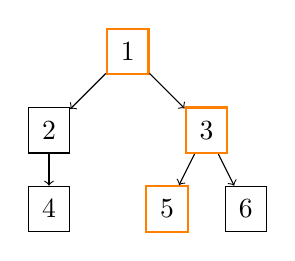
\begin{tikzpicture}
[dot/.style={rectangle,draw=black,fill=white,inner sep=5pt,minimum size=5pt}]
\node[dot,draw=orange,thick] at (0,5) (n1) {1};
\node[dot] at (-1,4) (n2) {2};
\node[dot,draw=orange,thick] at (1,4) (n3) {3};
\node[dot] at (-1,3) (n4) {4};
\node[dot,draw=orange,thick] at (0.5,3) (n5) {5};
\node[dot] at (1.5,3) (n6) {6};
\draw[->] (n1) -- (n2);
\draw[->] (n1) -- (n3);
\draw[->] (n2) -- (n4);
\draw[->] (n3) -- (n5);
\draw[->] (n3) -- (n6);
\end{tikzpicture}
\end{center}
\begin{itemize}\itemsep=8pt
    \item $\mathcal G = \{ \{4\}, \textcolor{orange}{\{5\}}, \{6\}, \{2,4\}, 
        \textcolor{orange}{\{3,5,6\}}, \textcolor{orange}{\{1,2,3,4,5,6\} \}}$
\item nonzero variables form a rooted and connected subtree
    \begin{itemize}
        \item if node is selected, so are its ancestors
        \item if node is not selected, neither are its descendants
    \end{itemize}
\end{itemize}
\end{frame}





\begin{frame}{Algorithm}
    if $L$ is not known (usually the case), can use the following line search:
    \noindent\rule[-5pt]{\textwidth}{0.4pt}
    {\footnotesize
    \begin{tabbing}
        {\bf given} $x^k$, $\lambda^{k-1}$, and parameter $\beta \in (0,1)$. \\*[\smallskipamount]
        Let $\lambda := \lambda^{k-1}$. \\*[\smallskipamount]
        {\bf repeat} \\
        \qquad \= 1.\ Let $z := \prox_{\lambda g}(x^{k} - \lambda \nabla f(x^{k}))$. \\
        \> 2.\ {\bf break if} $f(z) \leq \hat{f}_{\lambda}(z, x^{k})$. \\
        \> 3.\ Update $\lambda := \beta \lambda$. \\*[\smallskipamount]
        {\bf return} $\lambda^{k} := \lambda$, $x^{k+1}:=z$.
    \end{tabbing}}
    \noindent\rule[10pt]{\textwidth}{0.4pt}

    typical value of $\beta$ is $1/2$, and 
    \[
    \hat{f}_\lambda(x,y) = f(y) + \nabla f(y)^T (x - y) + 
    (1/2\lambda)\|x - y\|_2^2
    \]
\end{frame}


\end{document}